\documentclass[10pt,twocolumn]{article}

\usepackage[letterpaper,top=0.68in,bottom=0.72in,left=0.66in,right=0.66in,columnsep=0.23in]{geometry}
\usepackage[T1]{fontenc}
\usepackage{lmodern}
\usepackage{microtype}
\usepackage{amsmath,amssymb}
\usepackage{booktabs}
\usepackage{array}
\usepackage{enumitem}
\usepackage{xcolor}
\usepackage{graphicx}
\usepackage{tikz}
\usetikzlibrary{arrows.meta,positioning,fit,calc,shapes.geometric}
\usepackage{pgfplots}
\pgfplotsset{compat=1.18}
\usepackage{url}
\usepackage[hidelinks]{hyperref}
\usepackage[nameinlink,noabbrev]{cleveref}
\usepackage{balance}
\hypersetup{
  pdftitle={Budgeted Entanglement Routing for Sequential Multi-Agent Reinforcement Learning},
  pdfauthor={Anonymous Authors},
  pdfsubject={Scarce entanglement allocation in sequential multi-agent reinforcement learning},
  pdfkeywords={quantum MARL, entanglement allocation, nonlocal games, dynamic matching}
}

\definecolor{berblue}{RGB}{45,102,172}
\definecolor{bergreen}{RGB}{51,148,93}
\definecolor{berorange}{RGB}{230,126,34}
\definecolor{bergray}{RGB}{90,90,90}
\newcommand{\method}{\textsc{BER-MARL}}
\newcommand{\xor}{\mathbin{\oplus}}
\newcommand{\R}{\mathbb{R}}
\setlist{nosep,leftmargin=*}
\setlength{\textfloatsep}{7pt plus 2pt minus 2pt}
\setlength{\floatsep}{6pt plus 2pt minus 2pt}
\setlength{\intextsep}{6pt plus 2pt minus 2pt}

\title{Budgeted Entanglement Routing for Sequential\\Multi-Agent Reinforcement Learning}
\author{Anonymous Authors\\Anonymous Institution\\\texttt{anonymous@example.org}}
\date{}

\begin{document}
\maketitle

\begin{abstract}
Entanglement-assisted multi-agent learning usually treats entanglement as fixed or continuously available. We instead study a sequential resource problem in which four decentralized agents share six consumable Bell pairs over ten rounds of changing private-information coordination requests. Before private inputs arrive, a public controller must select a feasible matching of agent pairs to receive entanglement. We introduce \method, a masked Deep Q-Network that learns whether to spend or save Bell pairs from public request values, graph structure, budget, and horizon. Every request is a three-input binary-output XOR game. Its zero-communication classical value is obtained by exhaustive enumeration, while its Bell-assisted value is independently bounded by a semidefinite program. In a locked evaluation with 16 training seeds and 1,000 paired held-out sequences per seed, \method{} achieved mean entanglement surplus $0.5064$, compared with $0.3084$ for myopic greedy, $0.2268$ for random, and $0.2248$ for static allocation. The paired \method-minus-greedy difference was $0.1980$, with 95\% bootstrap interval $[0.1914,0.2043]$; all seeds were positive. \method{} recovered 88.66\% of the exact online dynamic-programming surplus. A preregistered condition requiring the one-sided lower bound to exceed 90\% failed because the bound was 87.68\%. The supported contribution is therefore a certified scarce-entanglement routing benchmark and robust learned allocation gain, rather than a near-oracle, hardware, or computational-advantage claim.
\end{abstract}

\noindent\textbf{Keywords:} quantum multi-agent reinforcement learning; entanglement allocation; nonlocal games; constrained reinforcement learning; dynamic matching.

\section{Introduction}
Entanglement can strengthen correlations between separated agents without revealing their private inputs \cite{bell1964einstein,clauser1969proposed,tsirelson1980quantum}. Existing entanglement-assisted multi-agent learning work demonstrates that such correlations can be incorporated into learned decentralized policies \cite{derieux2025eqmarl}. A separate systems question arises when entanglement is scarce: if many agent pairs could benefit but only a few Bell pairs are available, which opportunities should receive them, and when should the resource be saved?

We formulate this as a finite-horizon resource-allocation problem. Four agents face a changing public graph of pairwise coordination requests. Each endpoint later receives a private input and returns one binary output. An allocator chooses a matching before those private inputs arrive. Selected edges use frozen Bell-assisted local policies and consume one Bell pair each; unselected edges use exact optimal zero-message classical policies. The controller begins with six pairs for ten rounds.

This decomposition separates two questions. At the \emph{request level}, exhaustive classical enumeration and an XOR-game semidefinite program (SDP) certify how much one Bell pair can improve expected success. At the \emph{sequence level}, reinforcement learning decides when and where to spend the certified resource. The resulting method, \method{} (Budgeted Entanglement Routing for MARL), uses a masked Deep Q-Network (DQN) \cite{mnih2015human} over feasible graph matchings.

Our contributions are:
\begin{enumerate}
  \item a sequential benchmark for routing consumable entanglement over a dynamic matching-constrained multi-agent graph;
  \item exact request-level classical values and independent SDP certification of Bell-assisted values;
  \item \method, a public-information DQN allocator that learns budget pacing without private-context access;
  \item a prospective held-out comparison against random, static, myopic greedy, exact online dynamic programming (DP), and privileged ceilings; and
  \item complete raw results and an independent audit preserving both a strong learned-versus-greedy result and a failed near-oracle gate.
\end{enumerate}

\begin{figure*}[t]
\centering
\resizebox{0.98\textwidth}{!}{%
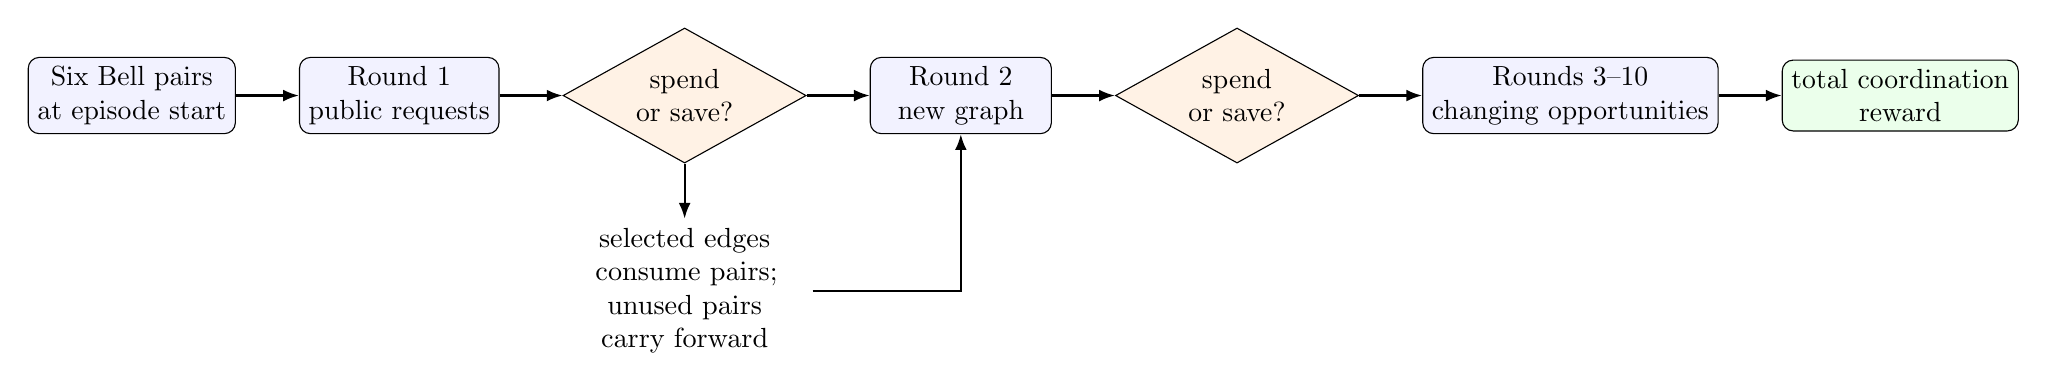
\begin{tikzpicture}[
  node distance=7mm and 8mm,
  box/.style={draw,rounded corners,minimum height=8mm,minimum width=23mm,align=center,fill=blue!5},
  decision/.style={draw,diamond,aspect=1.8,align=center,fill=orange!10},
  arr/.style={-{Latex[length=2mm]},thick}
]
\node[box] (budget) {Six Bell pairs\\at episode start};
\node[box,right=of budget] (r1) {Round 1\\public requests};
\node[decision,right=of r1] (d1) {spend\\or save?};
\node[box,right=of d1] (r2) {Round 2\\new graph};
\node[decision,right=of r2] (d2) {spend\\or save?};
\node[box,right=of d2] (rn) {Rounds 3--10\\changing opportunities};
\node[box,right=of rn,fill=green!8] (reward) {total coordination\\reward};
\draw[arr] (budget)--(r1); \draw[arr] (r1)--(d1); \draw[arr] (d1)--(r2);
\draw[arr] (r2)--(d2); \draw[arr] (d2)--(rn); \draw[arr] (rn)--(reward);
\node[below=7mm of d1,align=center,text width=30mm] (note) {selected edges consume pairs; unused pairs carry forward};
\draw[arr] (d1)--(note); \draw[arr] (note.east)-| (r2.south);
\end{tikzpicture}
}
\caption{The sequential allocation problem. A myopic policy spends on the best visible requests. A long-horizon policy may preserve Bell pairs for rarer, higher-value future states.}
\label{fig:timeline}
\end{figure*}

\section{Related Work and Positioning}
Bell nonlocality and quantum XOR games establish that entangled strategies can outperform local classical correlations under restricted communication \cite{bell1964einstein,clauser1969proposed,tsirelson1980quantum,cleve2004consequences}. This paper does not propose a new Bell inequality. It uses heterogeneous small XOR games as exactly certifiable demand units.

Quantum multi-agent reinforcement learning has considered entangled value functions and policies in repeated coordination environments. In particular, eQMARL studies distributed cooperation over quantum channels \cite{derieux2025eqmarl}. Our focus differs: local request policies are frozen before allocator training, Bell pairs are explicitly consumable, a graph matching limits simultaneous allocations, and the primary learned object is the long-horizon resource controller.

The allocator is related to constrained reinforcement learning and finite-horizon resource scheduling \cite{sutton2018reinforcement,mnih2015human}. DQN is used because the registered action set is discrete and small. PPO \cite{schulman2017proximal}, recurrent policies, model-based RL, and combinatorial action architectures are important future baselines. A bounded novelty screen found no retrieved study combining consumable Bell-pair budgets, dynamic matching constraints, decentralized request rewards, and a learned long-horizon allocator. We therefore avoid an unqualified priority claim pending a systematic human-reviewed literature search.

\section{Game Setting}
\subsection{One private-information request}
Each endpoint privately observes $x,y\in\{0,1,2\}$ and emits one bit $a,b\in\{0,1\}$. A public predicate $f:\{0,1,2\}^2\rightarrow\{0,1\}$ defines success:
\begin{equation}
  a\xor b=f(x,y).
  \label{eq:parity}
\end{equation}
The outputs are abstract coordination answers. They do not move a robot or select a physical channel in the implemented benchmark. Their purpose is to measure whether separated agents can satisfy a joint rule without sharing private inputs.

For example, if $f(1,2)=1$, both $(a,b)=(0,1)$ and $(1,0)$ win; neither agent is assigned a particular bit. If $f(1,2)=0$, both $(0,0)$ and $(1,1)$ win. A single input pair is trivial, but the agents must use one local rule over all nine input pairs. Conflicting cells can prevent perfect local play. For example, requiring ``same'' for $(0,0),(0,1),(1,0)$ and ``different'' for $(1,1)$ is inconsistent with fixed deterministic local outputs.

The input pair is sampled from a public, nonuniform positive weight matrix $w_{xy}$. For deterministic local functions $g,h$, expected success is
\begin{equation}
 V(g,h)=\sum_{x,y}w_{xy}\,\mathbf{1}\!\left[g(x)\xor h(y)=f(x,y)\right].
\end{equation}
There are eight binary functions of a three-valued input, hence only $8\times8=64$ deterministic pairs. We enumerate all of them:
\begin{equation}
 V_C=\max_{g,h}V(g,h).
 \label{eq:classical}
\end{equation}
Shared classical randomness cannot exceed this optimum because expected reward is linear in a mixture of deterministic strategies.

\subsection{Bell-assisted request policy}
On a selected edge, endpoints share
\begin{equation}
 |\Phi^+\rangle=\frac{|00\rangle+|11\rangle}{\sqrt{2}}.
\end{equation}
Each endpoint chooses a local binary measurement from its own private input. Six measurement angles are optimized to obtain $V_Q$. An independent XOR-game SDP supplies an upper bound on the quantum bias \cite{cleve2004consequences,tsirelson1980quantum}; the optimized policies match the bound to registered tolerance.

With urgency $u_e$, the certified expected gain from spending one Bell pair on request $e$ is
\begin{equation}
 G_e=u_e\max(0,V_{Q,e}-V_{C,e}).
 \label{eq:gain}
\end{equation}
Zero-gap requests remain in the family, so entangling every active edge is not automatically useful.

\begin{figure}[t]
\centering
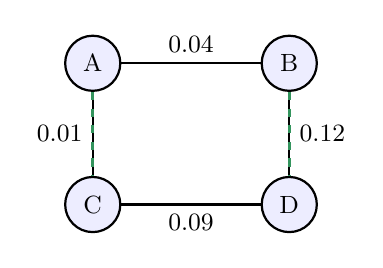
\begin{tikzpicture}[scale=0.78,
 agent/.style={circle,draw,thick,minimum size=7mm,fill=blue!7},
 edge/.style={thick}, every node/.style={font=\small}]
\node[agent] (A) at (0,2.3) {A};
\node[agent] (B) at (3.2,2.3) {B};
\node[agent] (C) at (0,0) {C};
\node[agent] (D) at (3.2,0) {D};
\draw[edge] (A)--node[above]{0.04}(B);
\draw[edge] (A)--node[left]{0.01}(C);
\draw[edge] (B)--node[right]{0.12}(D);
\draw[edge] (C)--node[below]{0.09}(D);
\draw[very thick,bergreen,dashed] (A)--(C);
\draw[very thick,bergreen,dashed] (B)--(D);
\end{tikzpicture}
\caption{Example public request graph. Edge labels are certified immediate gains. The dashed matching $\{A\!-!C,B\!-!D\}$ is feasible; allocations sharing an endpoint are not. Immediate gain alone may still be inferior to saving budget.}
\label{fig:graph}
\end{figure}

\subsection{Ten-round allocation problem}
The environment has four agents, ten rounds, and an initial budget $B_1=6$. Three to five of the six possible edges are active per round. Each active edge carries a request type and urgency. The public graph state follows a committed Markov transition matrix.

Before private inputs arrive, the allocator observes the public graph, gains, time, and budget. It selects a matching $M_t$ of active edges satisfying $|M_t|\leq B_t$. Selected edges use frozen Bell policies; other edges use frozen exact-classical policies. An agent may answer multiple requests classically but cannot receive entanglement on multiple edges in one round.

The immediate surplus and budget transition are
\begin{align}
 r_t &= \sum_{e\in M_t}G_e, \\
 B_{t+1} &= B_t-|M_t|.
\end{align}
The primary outcome is $S=\sum_{t=1}^{10}r_t$, equal to total expected return minus exact classical return on the same public sequence. The implementation integrates over private-input distributions using certified $V_C$ and $V_Q$; individual contexts are not sampled during allocator learning. This isolates scheduling from local-game sampling noise.

\section{Proposed Method: BER-MARL}
The state vector contains six current edge gains, six activity indicators, normalized budget, and normalized remaining horizon. A two-layer multilayer perceptron with 64 units per layer outputs Q values for ten global actions: the empty matching, six single edges, and three disjoint two-edge matchings. A deterministic mask removes inactive, endpoint-conflicting, and over-budget actions.

\begin{figure}[t]
\centering
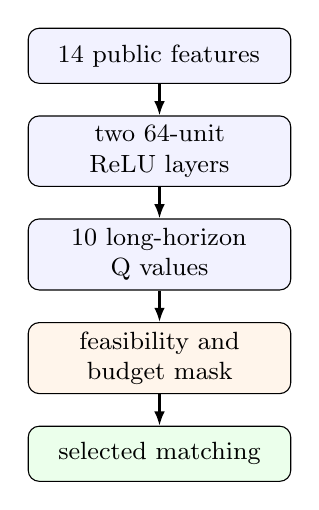
\begin{tikzpicture}[node distance=4mm,
 box/.style={draw,rounded corners,minimum height=7mm,align=center,text width=31mm,fill=blue!5},
 arr/.style={-{Latex[length=1.8mm]},thick}, every node/.style={font=\small}]
\node[box] (f) {14 public features};
\node[box,below=of f] (h) {two 64-unit ReLU layers};
\node[box,below=of h] (q) {10 long-horizon Q values};
\node[box,below=of q,fill=orange!8] (m) {feasibility and budget mask};
\node[box,below=of m,fill=green!8] (a) {selected matching};
\draw[arr] (f)--(h); \draw[arr] (h)--(q); \draw[arr] (q)--(m); \draw[arr] (m)--(a);
\end{tikzpicture}
\caption{\method{} architecture. The network receives no private endpoint context.}
\label{fig:architecture}
\end{figure}

For transition $(s_t,a_t,r_t,s_{t+1})$, DQN minimizes a Huber loss between $Q_\theta(s_t,a_t)$ and
\begin{equation}
 y_t=r_t+\max_{a'\in\mathcal{A}_{\mathrm{feas}}(s_{t+1})}Q_{\bar\theta}(s_{t+1},a'),
\end{equation}
using a replay buffer and target parameters $\bar\theta$. Training uses Adam at $5\times10^{-4}$, batch size 64, target updates every 200 optimizer steps, and 2,500 episodes per final seed. The endpoint policies are certified and frozen before DQN training; \method{} learns only resource allocation.

\section{Benchmarking Methods}
\begin{table*}[t]
\centering
\caption{Registered comparison methods. Random, static, greedy, and \method{} have identical public information, local policies, sequences, matching constraints, and six-pair budget.}
\label{tab:methods}
\small
\begin{tabular}{@{}lclp{8.6cm}@{}}
\toprule
Method & Bell budget & Future/model access & Role \\
\midrule
Classical exact & 0 & None & Defines zero surplus using exact optimal local strategies. \\
Quantum random & 6 & None & Tests whether arbitrary entanglement use is sufficient. \\
Quantum static & 6 & Non-test frequencies & Uses fixed edge priorities; does not respond to future value. \\
Quantum greedy & 6 & Current round & Selects the greatest visible certified gain; primary comparator. \\
\method{} & 6 & Learned experience & Proposed long-horizon public-information allocator. \\
Online DP & 6 & True transition matrix & Exact non-clairvoyant model-aware reference. \\
Future-clairvoyant & 6 & Realized future & Unattainable descriptive ceiling. \\
Message oracle & Not comparable & Private input exchange & Privileged information reference, excluded from fairness claims. \\
\bottomrule
\end{tabular}
\end{table*}

\paragraph{Classical exact.}
This method uses no Bell pairs. Every request is answered with the best zero-message deterministic local strategy from \cref{eq:classical}; its entanglement surplus is zero by definition. It establishes the return improved by quantum-assisted methods, but it is not an equal-resource allocator.

\paragraph{Quantum random.}
At each round, this control samples uniformly from the feasible matching set $\mathcal{M}(s_t,B_t)$. It has the same six-pair budget as \method{} but uses neither current request value nor future information. It tests whether arbitrary entanglement use is sufficient.

\paragraph{Quantum static.}
For each physical edge, a fixed priority is computed from non-test request frequencies and gains. Evaluation selects the feasible active matching with greatest total fixed priority. Priorities are not adapted to the final catalog. This tests whether a fixed deployment plan can replace sequential reasoning.

\paragraph{Quantum greedy.}
Greedy observes current certified gains and selects
\begin{equation}
M_t^{\mathrm{greedy}}=\arg\max_{M\in\mathcal{M}(s_t,B_t)}G(s_t,M).
\label{eq:greedy}
\end{equation}
It values present opportunities correctly but assigns zero value to preserving budget. It is the primary comparator because its principal difference from \method{} is long-horizon reasoning.

\paragraph{BER-MARL.}
The proposed method receives the same state, matching set, budget, and frozen request policies as greedy, but selects
\begin{equation}
M_t^{\mathrm{BER}}=\arg\max_{M\in\mathcal{M}(s_t,B_t)}Q_\theta(s_t,B_t,M).
\end{equation}
An improvement over greedy therefore measures learned budget pacing and anticipation of future public states rather than additional information.

\paragraph{Online dynamic programming.}
DP knows the exact held-out public transition matrix but not future random draws. Its recursion is
\begin{equation}
\begin{aligned}
J_t(s,b)=\max_{M\in\mathcal{M}(s,b)}\bigg[&G(s,M)\\
&+\sum_{s'}P(s'|s)J_{t+1}(s',b-|M|)\bigg].
\end{aligned}
\label{eq:dp}
\end{equation}
It is a privileged model-aware reference, not a learned equal-information competitor.

\paragraph{Future-clairvoyant reference.}
This method sees the complete realized ten-round sequence before acting and solves the sequence-specific budgeted matching problem. It is unattainable online and reports the remaining sequence-level headroom.

\paragraph{Message oracle.}
This reference lets endpoints exchange private inputs before acting, allowing joint outputs that satisfy every parity request. It solves a stronger-information problem and has no comparable Bell budget. We report it only as an information ceiling; it is excluded from the allocator claim and main chart.

The fair direct comparisons are \method{} versus random, static, and greedy. DP measures model-aware headroom. Future-clairvoyant and message oracles are descriptive ceilings, while classical exact defines zero surplus.

\section{Experimental Protocol}
The study was executed prospectively in five stages: plan and claims; request/task certification; bounded algorithm development and freeze; locked held-out evaluation; and independent release audit. Development considered four DQN configurations with two seeds each, followed by four fresh pilots. Before final access, the protocol fixed 16 training seeds, 2,500 training episodes per seed, 1,000 paired test sequences, final-checkpoint evaluation, 20,000 seed-level bootstrap resamples, and five positive-result gates.

Final models train on development and validation catalogs. Evaluation uses disjoint request types, a disjoint public transition catalog, and a disjoint sequence stream without adaptation. The independent training seed is the unit of inference; episodes within a seed are not treated as independent replicates.

The preregistered composite gate required: (i) a paired 95\% lower bound for \method-minus-greedy above zero; (ii) mean improvement at least 5\% of DP surplus; (iii) a one-sided 95\% lower bound for the \method/DP fraction above 0.90; (iv) a one-sided surplus lower bound above zero; and (v) no budget or matching violation.

\section{Results}
\begin{table}[t]
\centering
\caption{Held-out mean entanglement surplus.}
\label{tab:results}
\small
\begin{tabular}{@{}lr@{}}
\toprule
Method & Mean surplus \\
\midrule
Classical exact & 0.00000 \\
Quantum static & 0.22478 \\
Quantum random & 0.22685 \\
Quantum greedy & 0.30839 \\
\textbf{BER-MARL} & \textbf{0.50642} \\
Online DP & 0.57122 \\
Future-clairvoyant & 0.58326 \\
\bottomrule
\end{tabular}
\end{table}

\begin{figure}[t]
\centering
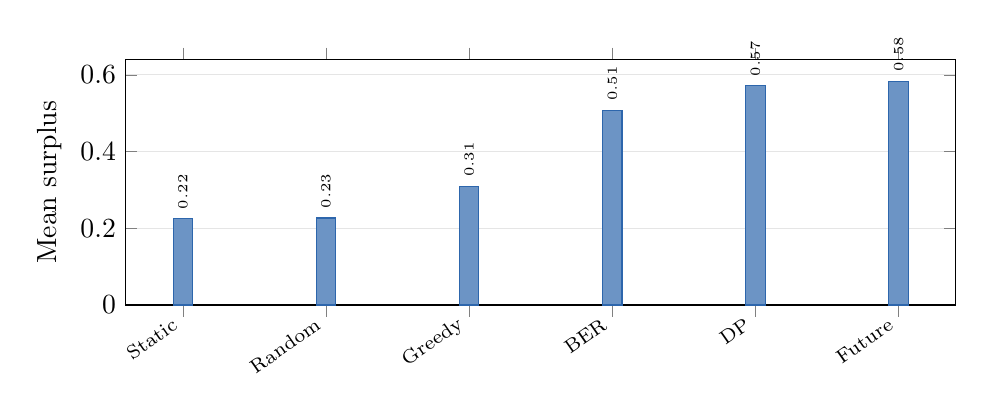
\begin{tikzpicture}
\begin{axis}[
  ybar, width=\columnwidth, height=4.7cm,
  ymin=0,ymax=0.64, ylabel={Mean surplus},
  symbolic x coords={Static,Random,Greedy,BER,DP,Future},
  xtick=data, x tick label style={rotate=35,anchor=east,font=\scriptsize},
  ymajorgrids=true, grid style={gray!20},
  bar width=7pt, nodes near coords,
  every node near coord/.append style={font=\tiny,rotate=90,anchor=west},
  enlarge x limits=0.08
]
\addplot[fill=berblue!70,draw=berblue] coordinates {
 (Static,0.22478) (Random,0.22685) (Greedy,0.30839)
 (BER,0.50642) (DP,0.57122) (Future,0.58326)};
\end{axis}
\end{tikzpicture}
\caption{Held-out surplus. \method{} closes most of the gap from greedy to model-aware DP.}
\label{fig:results}
\end{figure}

\method{} exceeded greedy by $0.19803$. The paired-seed 95\% bootstrap interval was $[0.19141,0.20432]$, and all 16 seeds were positive. Relative to greedy surplus, the increase was 64.2\%. Random and static allocation were nearly identical, showing that access to Bell pairs alone was insufficient. Greedy improved substantially over them, while \method{} added a further long-horizon gain.

\method{} recovered 88.66\% of online-DP surplus. Its one-sided 95\% lower bound was 87.68\%, below the registered 90\% requirement. Four of five gates passed; the composite gate failed solely on this near-oracle condition. No budget or matching violation occurred.

The twelve held-out request types had Bell-minus-classical gaps from zero to 0.03830, with mean 0.01760. Retaining zero-gap requests prevents the benchmark from rewarding indiscriminate entanglement use.

\subsection{Interpretation}
The ordering random/static $<$ greedy $<$ \method{} $<$ DP supports a specific mechanism. Immediate certified value matters, but future opportunity value and budget pacing add substantial reward. The remaining DP gap indicates incomplete zero-shot transfer to the new transition catalog. DP knows that catalog's exact transition matrix; \method{} receives no final-catalog adaptation period.

The classical-exact row defines surplus and intentionally uses no Bell pairs. It should not be interpreted as an equal-resource allocator baseline. Fair allocation comparisons are among random, static, greedy, \method, and DP.

\section{Audit, Reproducibility, and Resources}
An independent release program re-enumerated every held-out classical optimum, independently resolved every SDP ceiling, rebuilt all method means and bootstrap intervals from 23,000 raw episode rows, hashed all 16 checkpoints, and validated the authoritative bundles. Every reported scalar reproduced within $10^{-12}$.

The confirmatory run retained 16 checkpoints, 16,000 learned-policy episode records, all baseline records, request certificates, resolved configurations, resource counters, and failures. It consumed 600,000 allocator decisions, 552,592 optimizer updates including request certification, 1,382,400 analytic circuit-equivalent evaluations, zero physical shots, and 956.91 wall-seconds on CPU. A fresh remote clone validated 281 reportable bundles, and the repository test suite contained 128 passing tests.

\section{Limitations and Publication Scope}
The outputs are abstract coordination bits, not actions in a deployed network or robot team. This abstraction enables exact certification but limits application validity. Bell correlations are ideal and analytic; the confirmatory study does not include finite shots, hardware noise, or entanglement-generation failures. The graph has four agents and a small enumerated matching action set. PPO, recurrent, threshold, and learned-model allocators were not locked primary baselines. Finally, the novelty screen was bounded and does not justify an unqualified ``first'' claim.

The current evidence supports a preprint and workshop submission. A selective conference or journal version should add: (i) systematic related work; (ii) application-grounded action semantics; (iii) finite-shot and noisy-resource experiments; (iv) PPO, model-based, recurrent, and threshold controls; (v) scaling over agents, horizons, and budgets; and (vi) a prospectively frozen online-adaptation study addressing the observed DP gap. A small hardware demonstration would further strengthen the quantum-systems claim.

\section{Conclusion}
We introduced a certified sequential benchmark for allocating consumable entanglement across a changing multi-agent graph and proposed \method, a masked DQN resource controller using only public pre-context information. On held-out request types, dynamics, and sequences, \method{} increased entanglement surplus by 64.2\% over myopic greedy, with every one of 16 seeds positive and a paired 95\% interval excluding zero. Exact classical enumeration, independent SDP bounds, paired evaluation, retained failures, and a separate audit support this conclusion.

The claim has a clear boundary. \method{} recovered 88.66\% of model-aware DP value, but the preregistered one-sided lower bound did not exceed 90\%; we reject a near-oracle transfer claim. The contribution is not a new proof of Bell nonlocality. It is the formulation, certification, and empirical solution of a scarce-entanglement routing problem. The strongest next step is to give the abstract actions application semantics and combine public-model adaptation with realistic noisy quantum resources.

\balance
\bibliographystyle{plain}
\bibliography{BUDGETED_ENTANGLEMENT_ROUTING}

\end{document}
